\documentclass{beamer}

\usetheme{Frankfurt}

\usepackage[utf8]{inputenc}
\usepackage[T1]{fontenc}
\usepackage[frenchb]{babel}

\title{DIAPORAMA DU PROJET DE RENDU 3D PAR LANCER DE RAYONS}
\date{04-MAI-2020}
\author{ ABBAD KAMEL - 21911536 \\
    BOUSADIA LAHCENE - 21911132 \\
    MARTIN MAXENCE - 21807030\\
 	MEYER ARTHUR - 21805134 \\ }
\institute{\textbf{\large Université de Caen Normandie\\
		 PROFESSEUR : G. Bonnet, C. Alec \\}}
\setbeamertemplate{navigation symbols}{}% pour enlever les symboles de navigation en bas de chaque page
\setbeamertemplate{footline}[frame number]%pour changer le pied de page par un affichage des numéros de slide

\begin{document}
\maketitle
\frametitle{Plan}
\tableofcontents
%--------------------
\section{Introduction}
\subsection{Présentation du projet}
	\begin{frame}
	\frametitle{Définition}
		\begin{block}{Définition du Lancer de rayons}
			Le ray traycing (lancer de rayons) est une technique de rendu de graphiques en trois dimensions avec des interactions lumineuses très complexes. Cela signifie que vous pouvez créer des images pleines de miroirs, de surfaces transparentes et d'ombres, avec des résultats étonnants comme on peut le voir dans la figure.
		\end{block}
	\end{frame}
%--------------------
\subsection{Spécification minimal demandé}
	\begin{frame}
	\frametitle{Spécification minimal demandé}
		\begin{block}{Objectif du projet}
	L'objectif de notre project est de faire une application qui prend un fichier décrivant une scène au format ".pov" et de créer l'image associé. Pour pouvoir afficher l'image on doit lire le fichier qui décris la scène puis y appliquer un lancé de rayons pour créer une image où chaque rayons est un pixel qui change de couleurs en fonction de l'acteur touché, de l'éclairage etc ... Pour ce faire nous devions utiliser un peu d' algèbre et de géométrie pour colorer correctement rayons (et donc pixels).
		\end{block}
	\end{frame}
%--------------------
\section{Structure générale du projet}
	\subsection{Arborescence des packages}
		\begin{frame}
		\frametitle{Arborescence des packages}
			\begin{block}{Hiérarchie générale}
			Dans notre projet on a crée un grand dossier <<Engine>> qui est le principal package qui est constitué de trois autres répertoires aussi.
			\end{block}	
			\begin{exampleblock}{Arbre des packages} 
				Une photo qui résume les packages crées dans notre projet.
				\begin{figure}[h]
                    \begin{center}
                    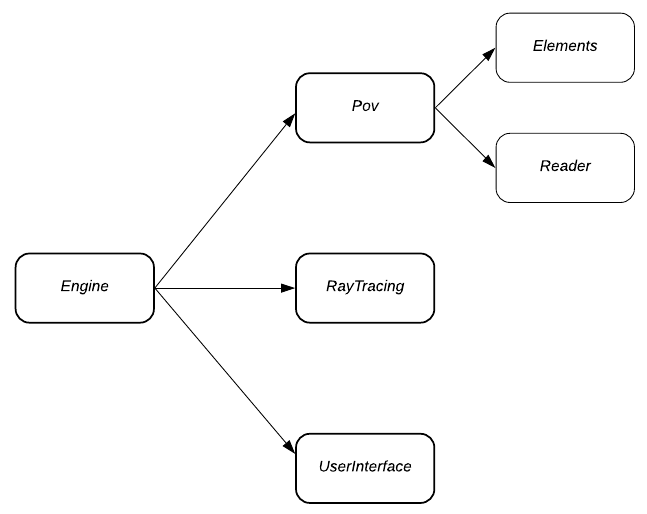
\includegraphics[width=0.3\textwidth]{./images/Arborescence.png}
                    \end{center}
                    \caption{Arborescence des packages.}
                    \label{fig}
                \end{figure}
			\end{exampleblock}	
		\end{frame}
	\subsection{Les packages utilisés}
		\begin{frame}
		\frametitle{Les packages utilisés}
			\begin{block}{Le role de chaque package}
				\begin{itemize}
					\item Le package POV qui se divise en deux packages <<Elements>> et <<Reader>>, on retrouve toutes les classes responsable des acteurs(formes géométriques), caméra et la lumière ainsi le chargement, sauvegardage et création des scènes.
					\item RayTracing est le deuxieme package qui gèrent les rayons et toutes les equations des vecteurs qui y sont associés.
					\item Enfin le package UserInterface qui est responsable de l'afffichage d'interface graphique (bouttons de sauvegarde, update, vue...), qui contient aussi la classe exécutable Main.
				\end{itemize}
			\end{block}
		\end{frame}
%--------------------
\section{Rendu final}
	\subsection{Diagramme UML}
		\begin{frame}
		\frametitle{UML du projet}
			\begin{block}{UML du Core}
			Diagramme général des classes qui représente le Core.
			\begin{figure}[h]
                    \begin{center}
                    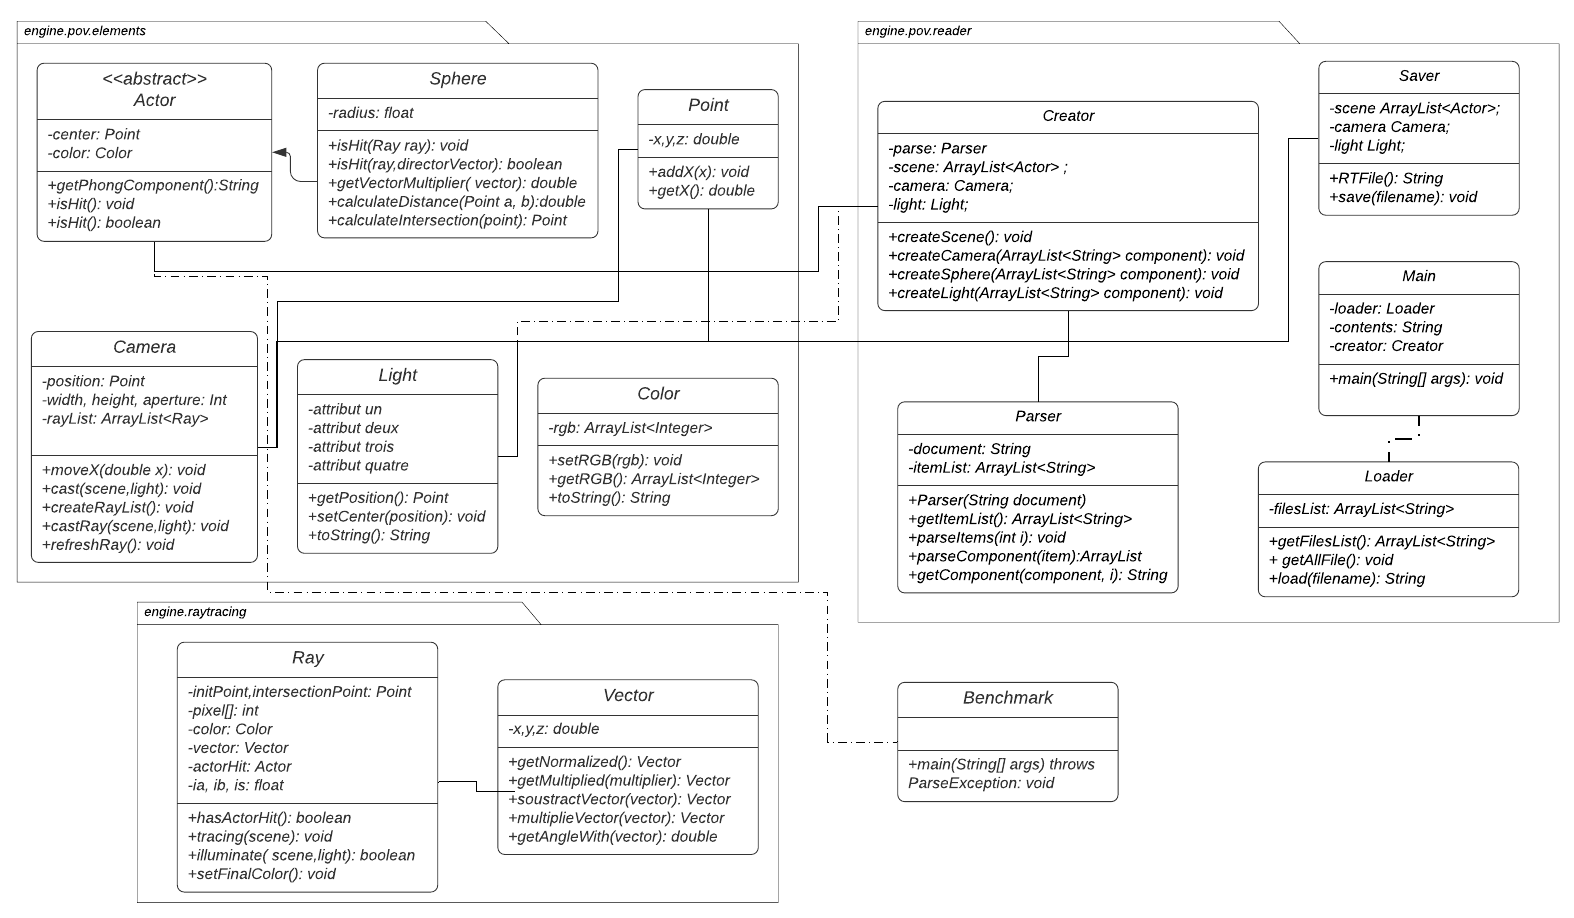
\includegraphics[width=1\textwidth]{./images/Core.png}
                    \end{center}
                    \label{fig}
            \end{figure}
			\end{block}
		\end{frame}
		\begin{frame}
			\begin{block}{UML de l'interface}
			Diagramme général des classes qui représente l'interface graphique.
			\begin{figure}[h]
                    \begin{center}
                    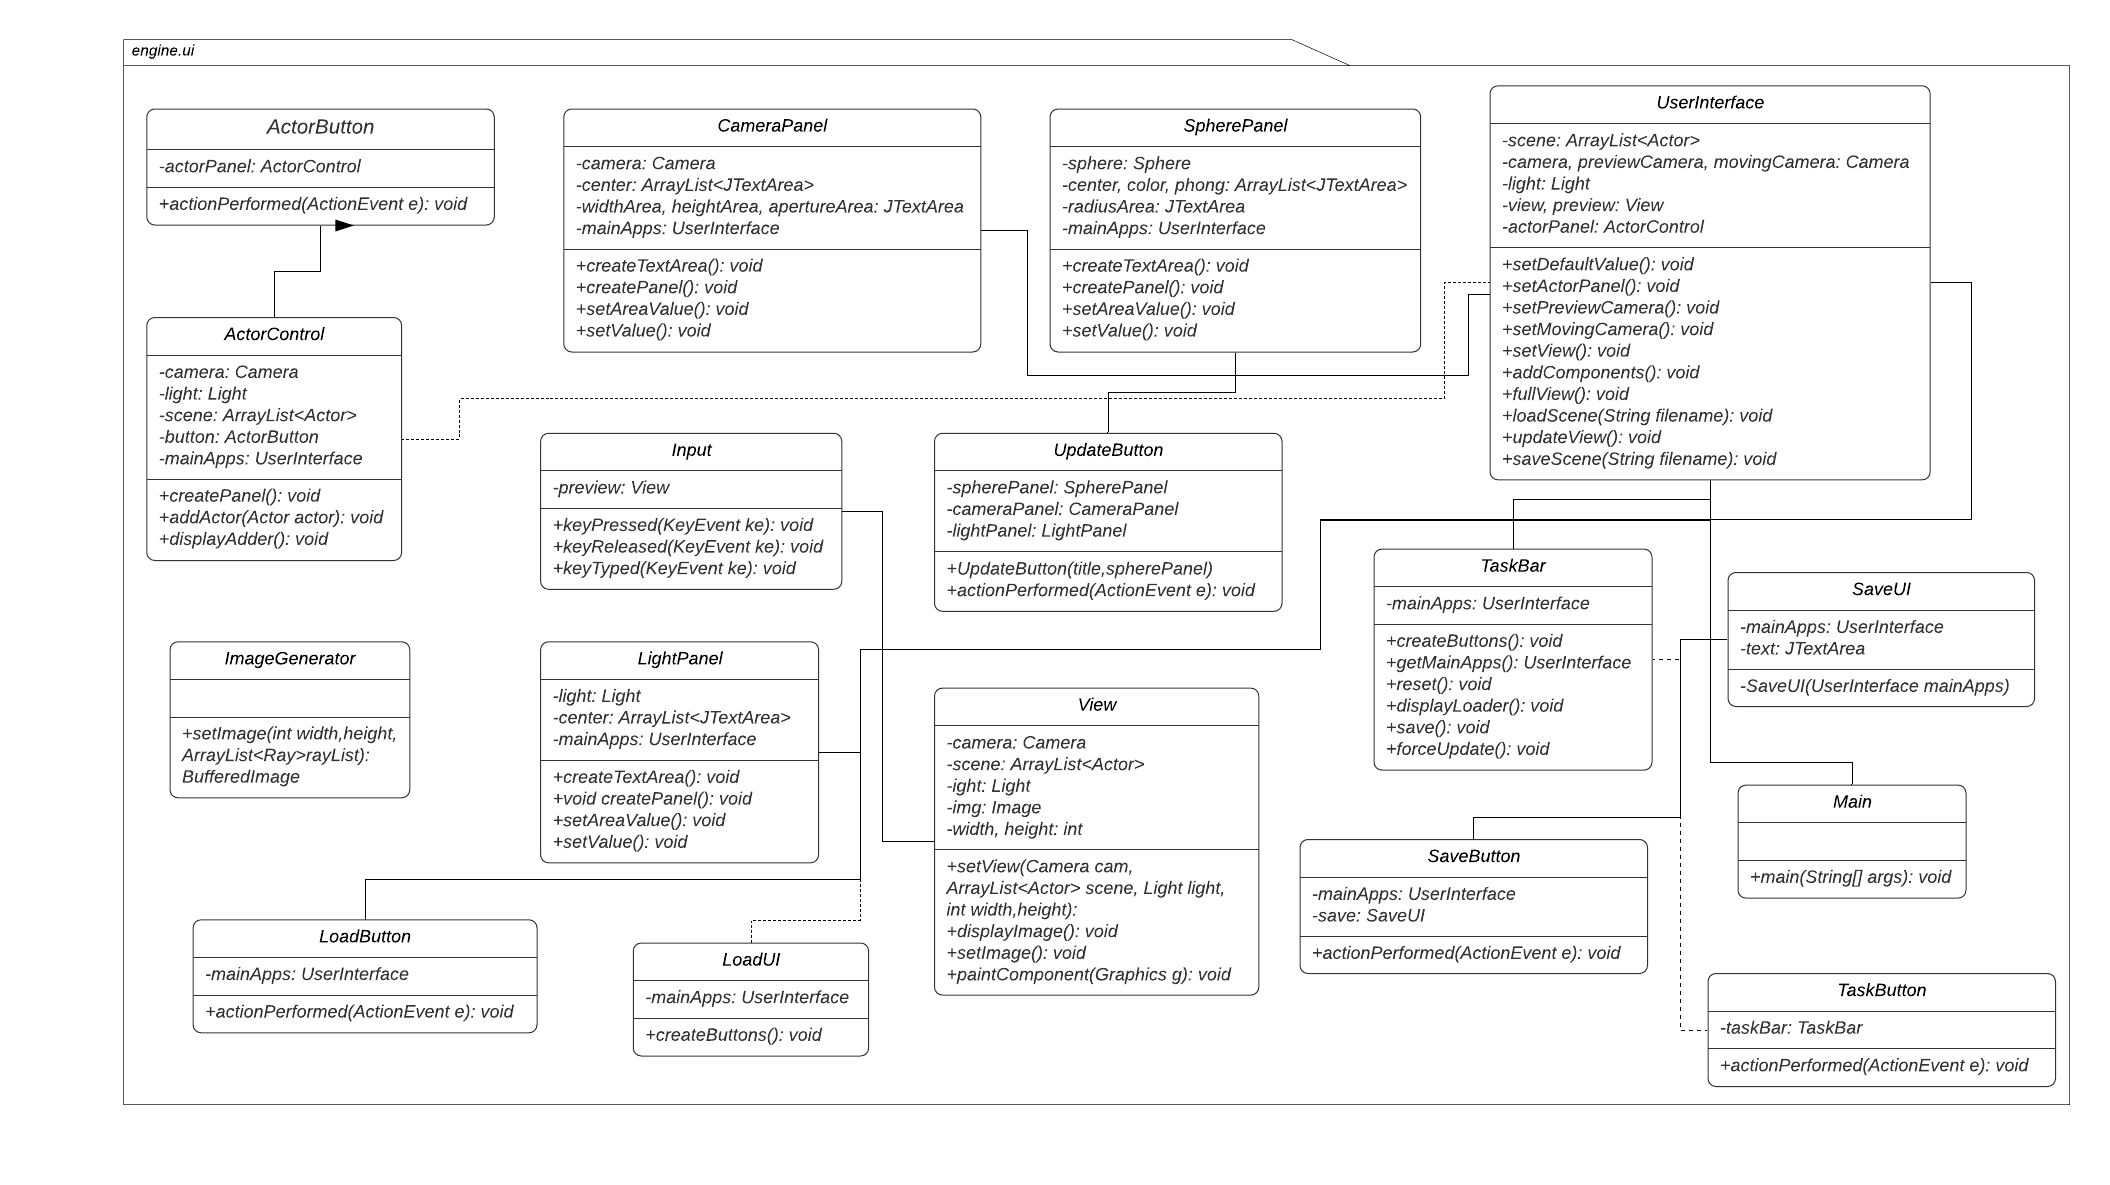
\includegraphics[width=1\textwidth]{./images/Interface.png}
                    \end{center}
                    \label{fig}
            \end{figure}
			\end{block}
		\end{frame}
	\subsection{Interface graphique}
		\begin{frame}
		\frametitle{Interface finale}
			\begin{block}{Version final}
					Image finale de l'interface graphique après l'éxecution.
			\begin{figure}[h]
                    \begin{center}
                    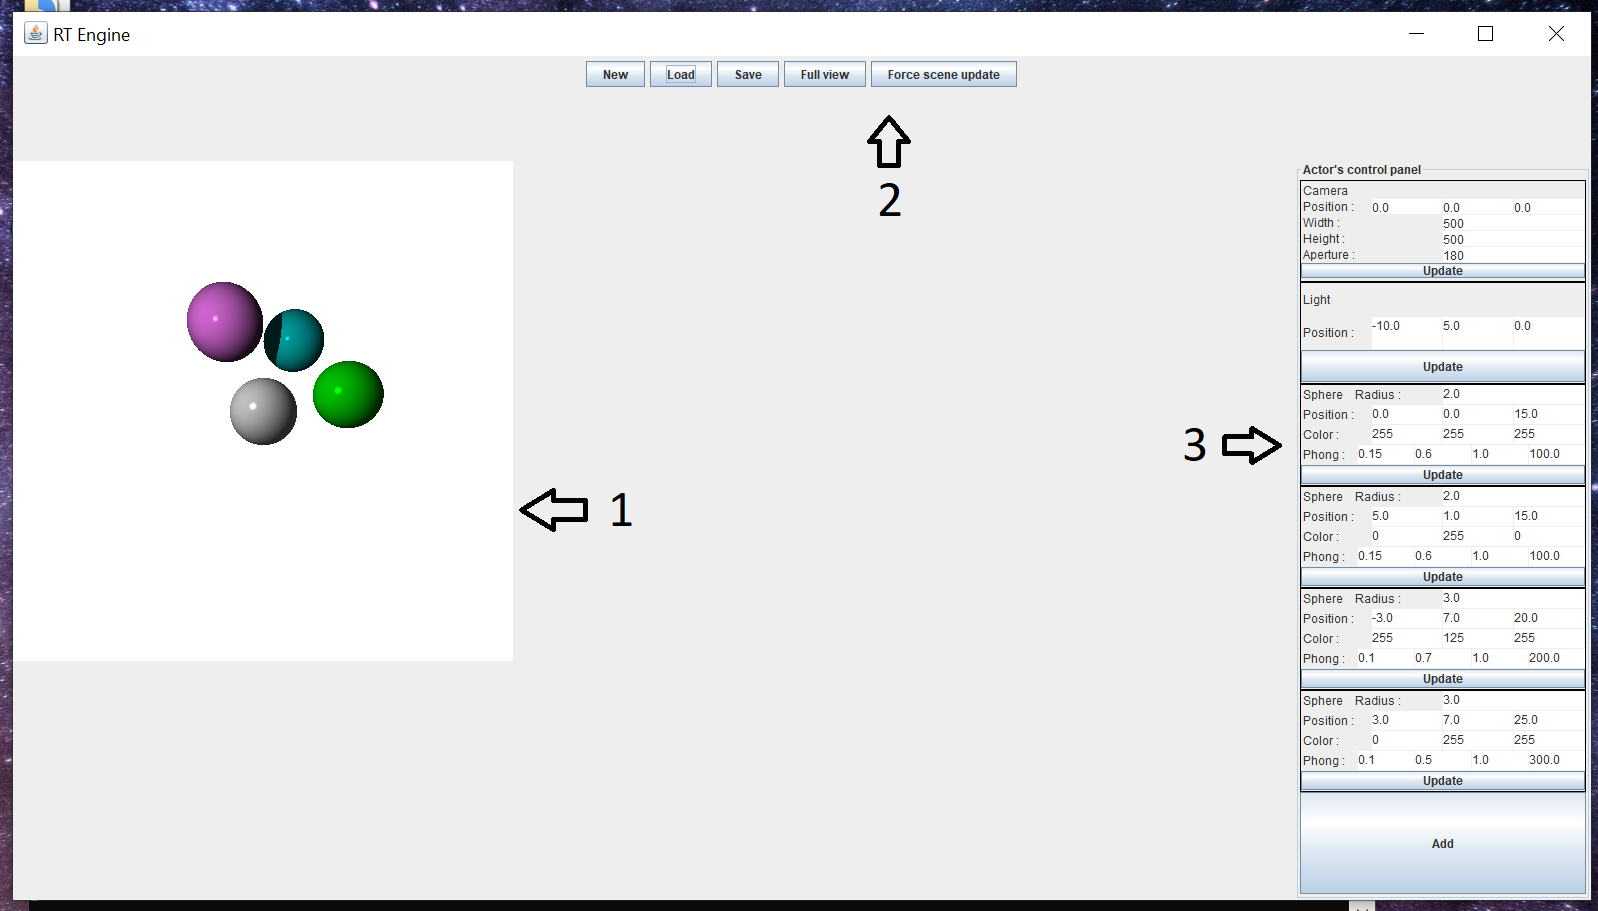
\includegraphics[width=1\textwidth]{./images/Capture.png}
                    \end{center}
                    \caption{Interface finale.}
                    \label{fig}
            \end{figure}
			\end{block}	
		\end{frame}
%--------------------
\section{Conclusion}
	\begin{frame}
		\frametitle{Conclusion}
			\begin{block}{Conclusion générale}
				\begin{itemize}
					\item L'objectif principal de ce projet est de réaliser une application en langage java en groupe permettant ainsi d'évoluer en travail d'équipe et de réaliser un moteur de rendu 3D.
					\item Nous avons un contenu limité avec l'affichage d'une forme unique qui est la sphère. D'autres formes auraient pu être implémenté tels que des cônes, des cylindres ou des cubes.
					\item De nombreuses fonctionnalités aurait pu être ajouté au projet tels que la rotation de la caméra et des acteurs, la réflection des objets entre eux ou l'ajout de transparence des objets (pour recrée des matière comme le metal avec une multiple réflection ou du verre pour la transparence.
				\end{itemize}
			\end{block}
		\end{frame}
\end{document}
